\documentclass[xcolor=table,aspectratio=43,dvipsnames]{beamer}
% \documentclass[xcolor=table]{beamer}
\usepackage{bm}
\usepackage[utf8]{inputenc}
% \usepackage[T1]{fontenc}
% \usepackage{cmbright}
% \usepackage[german, english]{babel} % required for rendering German special characters
\usepackage{booktabs}
\usepackage{color}
\usepackage{multicol}
\usepackage{siunitx} %pretty measurement unit rendering
\usepackage{multirow} %required for auto-generated tables http://www.tablesgenerator.com/
\usepackage[thinlines]{easytable}
\usepackage{hyperref} %enable hyperlink for urls
\usepackage{grffile} %determine file extension via LAST dot
\usepackage{soul} %strikethrough via \st{}
\usepackage[autoprint=false, gobble=auto, keeptemps=all, pyfuture=all]{pythontex} % create figures on-line directly from python!
\usepackage{graphviz}
\usepackage{minted}

\begin{pythontexcustomcode}[begin]{py}
import os, sys
almost_this_path = os.path.abspath(os.path.dirname(__file__))
this_path_base, _ = os.path.split(almost_this_path)
this_path = os.path.join(this_path_base,"pythontex")

from pylab import gcf
import matplotlib
import matplotlib.pyplot as plt

pytex.add_dependencies(os.path.join(this_path,'matplotlibrc.conf'))

plt.style.use(os.path.join(this_path,'matplotlibrc.conf'))

# Set the prefix used for figure labels
fig_label_prefix = 'fig'
# Track figure numbers to create unique auto-generated names
fig_count = 0

def figure_by_path(figure_path,textheight_frac=1,caption=None,label=None):
    latex_code = "\\begin{figure}\n"
    latex_code += "\\centering\\includegraphics[width={textheight_frac}\\textheight]{{{figure_path}}}\n".format(textheight_frac=textheight_frac,figure_path=figure_path)
    latex_code += "\\vspace{-2.5em}\n"
    latex_code += "\\caption{{{caption}}}\n".format(caption=caption)
    latex_code += "\\label{{fig:{label}}}\n".format(label=label)
    latex_code += "\\end{figure}\n"
    return latex_code

def save_fig(name='', legend=False, fig=None, ext='.pgf', fig_width=1, fig_height=1):
    '''
    Save the current figure (or `fig`) to file using `plt.save_fig()`.
    If called with no arguments, automatically generate a unique filename.
    Return the filename.
    '''
    # Get name (without extension) and extension
    if not name:
        global fig_count
        # Need underscores or other delimiters between `input_*` variables
        # to ensure uniqueness
        name = 'auto_fig_{}-{}'.format(pytex.id, fig_count)
        fig_count += 1
    else:
        if len(name) > 4 and name[:-4] in ['.pgf', '.svg', '.png', '.jpg']:
            name, ext = name.rsplit('.', 1)

    # Get current figure if figure isn't specified
    if not fig:
        fig = gcf()
    fig.set_size_inches(fig_width,fig_height)
    fig.savefig(name + ext)
    fig.clf()
    return name

def latex_environment(name, content='', option=''):
    '''
    Simple helper function to write the `\begin...\end` LaTeX block.
    '''
    return '\\vspace{-0.25cm}\\begin{%s}%s\n%s\n\\end{%s}' % (name, option, content, name)

def latex_figure(name=None, caption='', label='', width=1):
    ''''
    Auto wrap `name` in a LaTeX figure environment.
    Width is a fraction of `\textwidth`.
    '''
    if not name:
        name = save_fig()
    content = '\\centering\n'
    content += '\\makeatletter\\let\\input@path\\Ginput@path\\makeatother\n'
    content += '\\input{%s.pgf}\n' % name
    if not label:
        label = name
    if caption and not caption.rstrip().endswith('.'):
        caption += '.'
    if caption:
        # `\label` needs to be in `\caption` to avoid issues in some cases
        content += "\\caption{%s\\label{%s:%s}}\n" % (caption, fig_label_prefix, label)
    return latex_environment('figure', content, '[htp]')

pytex.bio_fignum = 0
#global pytex # try without this line
def bio_fig(gdd, fname=None, caption=None, label=None):
#        global pytex # and this one, should work
        if fname is None:
            fname = 'pythontex-files-pres/biopython_fig_{0}-{1}.pdf'.format(pytex.id, pytex.bio_fignum)
        gdd.write(fname, "PDF")
        template = '''
    \\begin{{figure}}
    \\centering
    \\includegraphics{{{fname}}}
    \\caption{{ {label} {caption} }}
    \\end{{figure}}
    '''
        if caption is None:
            caption = ''
        if label is None:
            label = ''
        else:
            if not label.startswith('fig:'):
                label = 'fig:' + label
            label = '\\label{{{0}}}'.format(label)
        template = template.format(fname=fname.rsplit('.', 1)[0], label=label, caption=caption)
        print(template)
        pytex.add_created(fname)
        pytex.bio_fignum += 1
        return template
\end{pythontexcustomcode}
\begin{pythontexcustomcode}[end]{py}
\end{pythontexcustomcode}

\begin{pythontexcustomcode}[begin]{py}
DOC_STYLE = 'slides/main.conf' 
pytex.add_dependencies(DOC_STYLE, 'slides/3dplot.conf')
\end{pythontexcustomcode}
 

\DeclareUnicodeCharacter{00A0}{ }
\setbeamersize{text margin left=0.8em,text margin right=0.8em}

\DeclareSIUnit\pixel{px}

\usecolortheme[RGB={199,199,199}]{structure}
\usetheme{Dresden}

\newenvironment{figurehere}
{\def\@captype{figure}}
{}
\makeatother

\definecolor{dy}{RGB}{202,202,0}
\definecolor{rsblue}{HTML}{00a3cc}
\definecolor{mg}{gray}{0.30}
\definecolor{lg}{gray}{0.60}
\definecolor{vlg}{gray}{0.78}
\definecolor{tlg}{gray}{0.88}

\setbeamercolor{caption name}{fg=lg}
\setbeamercolor{caption}{fg=lg}
\setbeamercolor{author}{fg=lg}
\setbeamercolor{institute}{fg=lg}
\setbeamercolor{date}{fg=lg}
\setbeamercolor{title}{fg=mg}
\setbeamertemplate{caption}{\centering\insertcaption\par}
\setbeamertemplate{navigation symbols}{}


\usepackage[british]{babel} % decent hyphenation, avoiding e.g. anal-ysis
\usepackage[iso]{isodate}
\usepackage{sansmath}
\usepackage{booktabs}
\usepackage{graphicx}
\usepackage{graphviz}
\usepackage{makecell}
\usepackage{minted}
\usepackage{siunitx}
\usepackage{subcaption}
\usepackage[section]{placeins}
\usepackage{amsfonts} % needed for \mathbb{} (Only works on capital letters!)
\usepackage{tikz}
\usetikzlibrary{shapes,snakes}
%\usetikzlibrary{shapes.geometric}

\usepackage{hyperref}
\usepackage{amsmath}
% Needs to be loaded after hyperref and amsmath
\usepackage{cleveref}

% new commands
\newcommand{\xdensity}{\textit{p}_x (\textbf{x})}
\newcommand{\udensity}{\textit{p}_u (\textbf{u})}
\newcommand{\transformer}{\tau(z_i;\textbf{h}_i)}
\newcommand{\conditioner}{c_i(\textbf{z}_{<1})}
\newcommand{\where}{\quad \text{where} \quad}
\newcommand{\xset}{\mathbb{X}}
\newcommand{\xseti}{\mathbb{X}^{(i)}}
\newcommand{\approxdistri}{q_{\phi_i}(\textbf{z}|\xseti)}
\newcommand{\approxdistr}{q_{\phi, \psi}(\textbf{z}|\xset)}
\newcommand{\truedistri}{p_{\theta}(\textbf{z}|\xseti)}
\newcommand{\truedistr}{p_{\theta}(\textbf{z}|\textbf{X})}
\newcommand{\elbo}{\mathcal{L}(\theta, \phi; \xseti)}
\newcommand{\xsubset}{\mathbb{X}_k}
\newcommand{\lmopoe}{\mathcal{L}_{MoPoE}(\theta, \phi; \xset)}
\newcommand{\powerset}{\mathcal{P}(\xset)}
\newcommand{\pFmean}{\mathcal{M}_{f_{\psi}}}
\newcommand{\DklTrueApprox}{D_{KL} \left( \approxdistr || \truedistr \right)}
\newcommand{\Mnfi}{\mathcal{M}_{f_{\psi}}\left( q_{\phi _i}(\textbf{z}|\textbf{x}_i) \right)}




% PythonTeX
\usepackage[autoprint=false, gobble=auto, keeptemps=all, pyfuture=all]{pythontex} % create figures on-line directly from python!
\usepackage{pgf}
\begin{pythontexcustomcode}[begin]{py}
import os, sys
almost_this_path = os.path.abspath(os.path.dirname(__file__))
this_path_base, _ = os.path.split(almost_this_path)
this_path = os.path.join(this_path_base,"pythontex")

from pylab import gcf
import matplotlib
import matplotlib.pyplot as plt

pytex.add_dependencies(os.path.join(this_path,'matplotlibrc.conf'))

plt.style.use(os.path.join(this_path,'matplotlibrc.conf'))

# Set the prefix used for figure labels
fig_label_prefix = 'fig'
# Track figure numbers to create unique auto-generated names
fig_count = 0

def figure_by_path(figure_path,textheight_frac=1,caption=None,label=None):
    latex_code = "\\begin{figure}\n"
    latex_code += "\\centering\\includegraphics[width={textheight_frac}\\textheight]{{{figure_path}}}\n".format(textheight_frac=textheight_frac,figure_path=figure_path)
    latex_code += "\\vspace{-2.5em}\n"
    latex_code += "\\caption{{{caption}}}\n".format(caption=caption)
    latex_code += "\\label{{fig:{label}}}\n".format(label=label)
    latex_code += "\\end{figure}\n"
    return latex_code

def save_fig(name='', legend=False, fig=None, ext='.pgf', fig_width=1, fig_height=1):
    '''
    Save the current figure (or `fig`) to file using `plt.save_fig()`.
    If called with no arguments, automatically generate a unique filename.
    Return the filename.
    '''
    # Get name (without extension) and extension
    if not name:
        global fig_count
        # Need underscores or other delimiters between `input_*` variables
        # to ensure uniqueness
        name = 'auto_fig_{}-{}'.format(pytex.id, fig_count)
        fig_count += 1
    else:
        if len(name) > 4 and name[:-4] in ['.pgf', '.svg', '.png', '.jpg']:
            name, ext = name.rsplit('.', 1)

    # Get current figure if figure isn't specified
    if not fig:
        fig = gcf()
    fig.set_size_inches(fig_width,fig_height)
    fig.savefig(name + ext)
    fig.clf()
    return name

def latex_environment(name, content='', option=''):
    '''
    Simple helper function to write the `\begin...\end` LaTeX block.
    '''
    return '\\vspace{-0.25cm}\\begin{%s}%s\n%s\n\\end{%s}' % (name, option, content, name)

def latex_figure(name=None, caption='', label='', width=1):
    ''''
    Auto wrap `name` in a LaTeX figure environment.
    Width is a fraction of `\textwidth`.
    '''
    if not name:
        name = save_fig()
    content = '\\centering\n'
    content += '\\makeatletter\\let\\input@path\\Ginput@path\\makeatother\n'
    content += '\\input{%s.pgf}\n' % name
    if not label:
        label = name
    if caption and not caption.rstrip().endswith('.'):
        caption += '.'
    if caption:
        # `\label` needs to be in `\caption` to avoid issues in some cases
        content += "\\caption{%s\\label{%s:%s}}\n" % (caption, fig_label_prefix, label)
    return latex_environment('figure', content, '[htp]')

pytex.bio_fignum = 0
#global pytex # try without this line
def bio_fig(gdd, fname=None, caption=None, label=None):
#        global pytex # and this one, should work
        if fname is None:
            fname = 'pythontex-files-pres/biopython_fig_{0}-{1}.pdf'.format(pytex.id, pytex.bio_fignum)
        gdd.write(fname, "PDF")
        template = '''
    \\begin{{figure}}
    \\centering
    \\includegraphics{{{fname}}}
    \\caption{{ {label} {caption} }}
    \\end{{figure}}
    '''
        if caption is None:
            caption = ''
        if label is None:
            label = ''
        else:
            if not label.startswith('fig:'):
                label = 'fig:' + label
            label = '\\label{{{0}}}'.format(label)
        template = template.format(fname=fname.rsplit('.', 1)[0], label=label, caption=caption)
        print(template)
        pytex.add_created(fname)
        pytex.bio_fignum += 1
        return template
\end{pythontexcustomcode}
\begin{pythontexcustomcode}[end]{py}
\end{pythontexcustomcode}

\begin{pythontexcustomcode}[begin]{py}
pytex.add_dependencies(
	'lib/utils.py',
	'lib/categorical.py',
	)
\end{pythontexcustomcode}
% Single-session PythonTeX codeblocks
\newcounter{pysessioncounter}
\newcommand{\sessionpy}{%
          \edef\sessionpysession{session\arabic{pysessioncounter}}%
            \stepcounter{pysessioncounter}%
              \expandafter\py\expandafter[\sessionpysession]}

% SIunitx customizations detect-all will use the current font for typesetting
\sisetup{per-mode=symbol, detect-all, range-units = single}
\newcommand\SIci[5]{\SI{#1}{#2}, {#3}CI: \SIrange{#4}{#5}{#2}}

% Fix for matplotlib PGF wonkiness which isn't interpreted correctly by pdflatex
\DeclareUnicodeCharacter{2212}{-}
\title[Reproducible Self-Publishing via Python\TeX\ --- Introduction and Reference Slides]{Reproducible Self-Publishing via Python\TeX}
\subtitle{Introduction and Reference Slides\\\href{https://github.com/TheChymera/RepSeP}{\small\texttt{[ github.com/TheChymera/RepSeP ]}}}
\author[Horea Christian]{Horea Christian\\\href{https://twitter.com/TheChymera}{\small\texttt{[ @TheChymera ]}}}
\institute{Institute for Biomedical Engineering, ETH and University of Zürich}
\begin{document}
	\begin{frame}
		\titlepage
	\end{frame}
	\section{Publishing}
		\subsection{Free and Open Scientific Publishing}
			\begin{frame}{Publish From Code, Openly.}
				\begin{itemize}
					\item Transparency $\longrightarrow$ verifiability.
					\item Reproducibility $\longrightarrow$ hackability.
					\item Version management support:
					\begin{itemize}
						\item \colorbox{tlg}{\texttt{diff}}-ability.
						\item \colorbox{tlg}{\texttt{blame}}-ability.
					\end{itemize}
				\end{itemize}
			\end{frame}
			\begin{frame}{Publish in a Distributed Model, Free.}
				\begin{itemize}
					\item No entry barrier $\longrightarrow$ citizen science.
					\item No institutional bias $\longrightarrow$ free science.
					\item \textit{Less} publication bias $\longrightarrow$ honest science.
					\item “Direct Market Access”.
				\end{itemize}
			\end{frame}
			\begin{frame}{Publish, in a Presentable Format.}
				\noindent\makebox[\textwidth][c]{%
					\begin{minipage}{.35\textwidth}
						\begin{itemize}
							\item Article.
							\item Poster.
							\item Slides.
						\end{itemize}
					\end{minipage}
					\begin{minipage}{.35\textwidth}
						\begin{figure}
							\centering
							
\includegraphics[width=0.6\textwidth]{img/pythontex.pdf}
						\end{figure}
					\end{minipage}
				}\vspace{3em}
				\centering (“Notebooks” integrate poorly with both presentation and development.)
			\end{frame}
	\section{Features}
		\subsection{Create All Graphic Elements Directly from Source.}
			\begin{frame}{}
				\py{pytex_fig('scripts/3dplot.py', conf='slides/3dplot.conf', label='3dplot', caption='A 3D plot.')}
			\end{frame}
			\begin{frame}{}
				\setlength\abovecaptionskip{-5pt}
				\py{pytex_fig('scripts/bsc_percentage.py', conf='slides/tall.conf', label='bsc_percentage', caption='Percentage of Bachelor’s degrees conferred to women in the U.S.A. by major (1970-2011).')}
			\end{frame}
			\begin{frame}{And So Much More}
				\py{pytex_subfigs(
					[
						{'script':'scripts/vc_violin.py', 'label':'vcv', 'conf':'slides/1col.conf', 'options_pre':'{.48\\textwidth}',
						},
						{'script':'scripts/vcc_violin.py', 'label':'vccv','conf':'slides/1col.conf', 'options_pre':'{.48\\textwidth}',
						},
						],
					environment='figure',
					label='fig:vc',
					)}
			\end{frame}
			\begin{frame}{}
				\begin{table}[]
					\vspace{0.4em}
						\py{
							pytex_tab(
								script='scripts/stim_table.py',
								label='sp',
								caption='BIDS event file table.',
								options_pre='\\centering \\resizebox{0.5\\textwidth}{!}{',
								data='data/JogB.tsv',
								options_post='}',
								)
							}
					\vspace{0.4em}
				\end{table}
			\end{frame}
			\begin{frame}{Sometimes Less is More}
				\centerline{\py{pytex_printonly('scripts/anova.py')}}
			\end{frame}
			\begin{frame}{But Sometimes You Just Want More}
				\begin{itemize}
					\item Processing Factor: \py{boilerplate.fstatistic('Processing', condensed=True)}
					\item Template Factor: \py{boilerplate.fstatistic('Template', condensed=True)}
					\item Processing:Template Intearction: \py{boilerplate.fstatistic('Processing:Template', condensed=True)}
				\end{itemize}
			\end{frame}
	\section{Source}
		\subsection{The Code, Workflow, and Environment Behind the Curtain}
			\begin{frame}[fragile]{Typesetting the Previous Radar Plot}
				\begin{minipage}{0.15\textwidth}~\end{minipage}
				\begin{minipage}{0.5\textwidth}
					\begin{pyverbatim}
						\py{
							pytex_fig('scripts/radar.py',
								label='radar',
								caption='A radar plot.',
								)
							}
					\end{pyverbatim}
				\end{minipage}
			\end{frame}
			\begin{frame}[fragile]{Typesetting the Previous Table}
				\begin{minipage}{0.15\textwidth}~\end{minipage}
				\begin{minipage}{0.5\textwidth}
					\begin{pyverbatim}
						\py{
							pytex_tab(
								script='scripts/stim_table.py',
								label='sp',
								caption='BIDS event file table.',
								options_pre='\\centering \\resizebox{0.5\\textwidth}{!}{',
								data='data/JogB.tsv',
								options_post='}',
								)
							}
					\end{pyverbatim}
				\end{minipage}
			\end{frame}
			\begin{frame}[fragile]{Typesetting the Previous Inline Statistic}
				\begin{minipage}{0.07\textwidth}~\end{minipage}
				\begin{minipage}{0.5\textwidth}
					\begin{pyverbatim}
						\py{
							pytex_printonly('scripts/drs_activityANOVA.py')
							}
					\end{pyverbatim}
				\end{minipage}
			\end{frame}
			\begin{frame}{The Framework Topology}
				\begin{minipage}{0.55\textwidth}
					\begin{itemize}
						\item Reduced information duplication.
						\item Continuous development support.
					\end{itemize}
				\end{minipage}
				\begin{minipage}{0.43\textwidth}
					\vspace{-3em}
					\begin{figure}
						\centering
						\includedot[width=0.9\textwidth]{data/topology}
					\end{figure}
				\end{minipage}
			\end{frame}
			\begin{frame}{The Workflow}
				\begin{itemize}
					\item Asynchronous offloading for time-consuming analysis.
					\item Separate packaging for deep analysis stacks.
				\end{itemize}
				\vspace{-2em}
				\begin{figure}
					\centering
					\includedot[width=\textwidth]{data/workflow}
				\end{figure}
			\end{frame}
			\begin{frame}{Minimal First-Level Dependencies}
				\inputminted[bgcolor=tlg,firstline=18,lastline=25]{bash}{.gentoo/app-text/repsep/repsep-99999.ebuild}
				Following the Package Manager Standard (PMS):
				\begin{itemize}
					\item Because dependency graphs should never be managed ad hoc.
				\end{itemize}
			\end{frame}
	\section{You}
		\subsection{How You Can Benefit from This Right Now.}
			\begin{frame}{Co-Author the Reference Implementation}
				\begin{itemize}
					\item The \colorbox{tlg}{\texttt{article.tex}} reference document is still in early draft.
					\item You can contribute, fork, and publish it however you want.
				\end{itemize}
			\end{frame}
			\begin{frame}{Gain the Best Exposure for Your most Underexposed Work}
				\begin{itemize}
					\item Pay-for-Paywall vs. “Direct Market Access”.
				\end{itemize}
				\begin{minipage}{0.49\textwidth}
					\begin{figure}
						\centering
						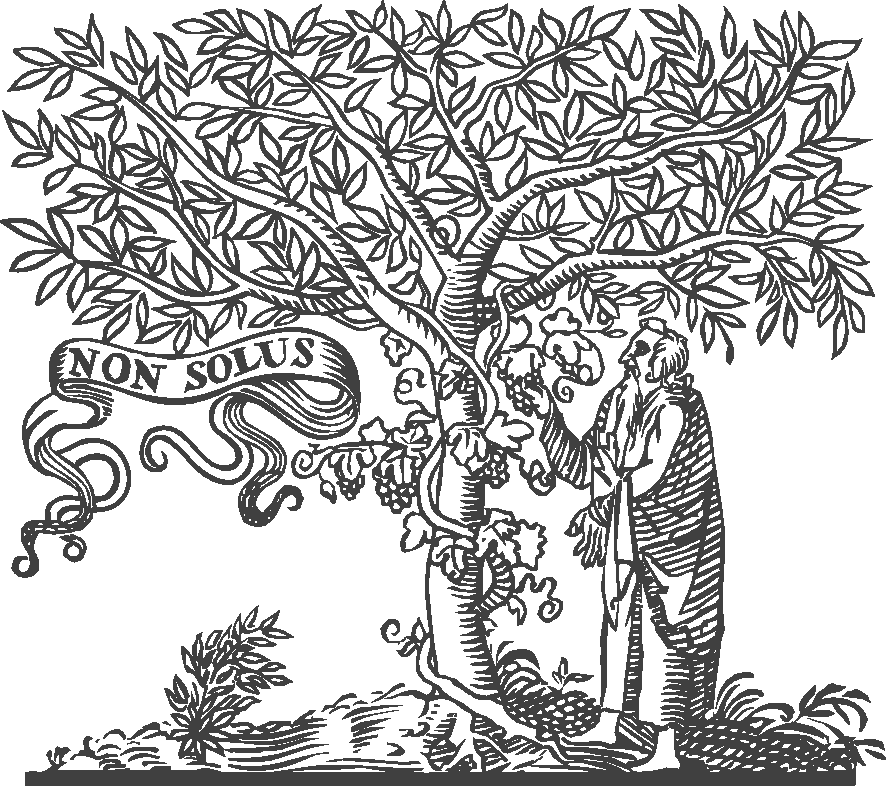
\includegraphics[width=0.8\textwidth]{img/elsevier.pdf}
					\end{figure}
				\end{minipage}
			\end{frame}
			\begin{frame}{Gain the Best Exposure for Your most Underexposed Work}
				\begin{itemize}
					\item Pay-for-Paywall vs. “Direct Market Access”.
				\end{itemize}
				\begin{minipage}{0.49\textwidth}
					\begin{figure}
						\centering
						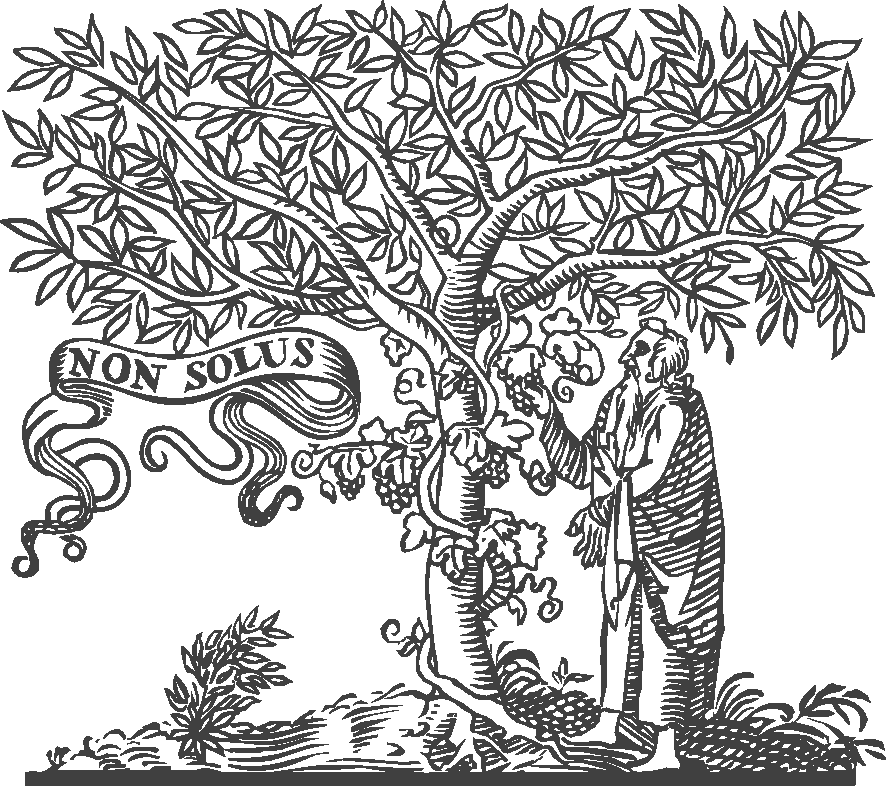
\includegraphics[width=0.8\textwidth]{img/elsevier.pdf}
					\end{figure}
				\end{minipage}
				\begin{minipage}{0.49\textwidth}
					\begin{figure}
						\centering
						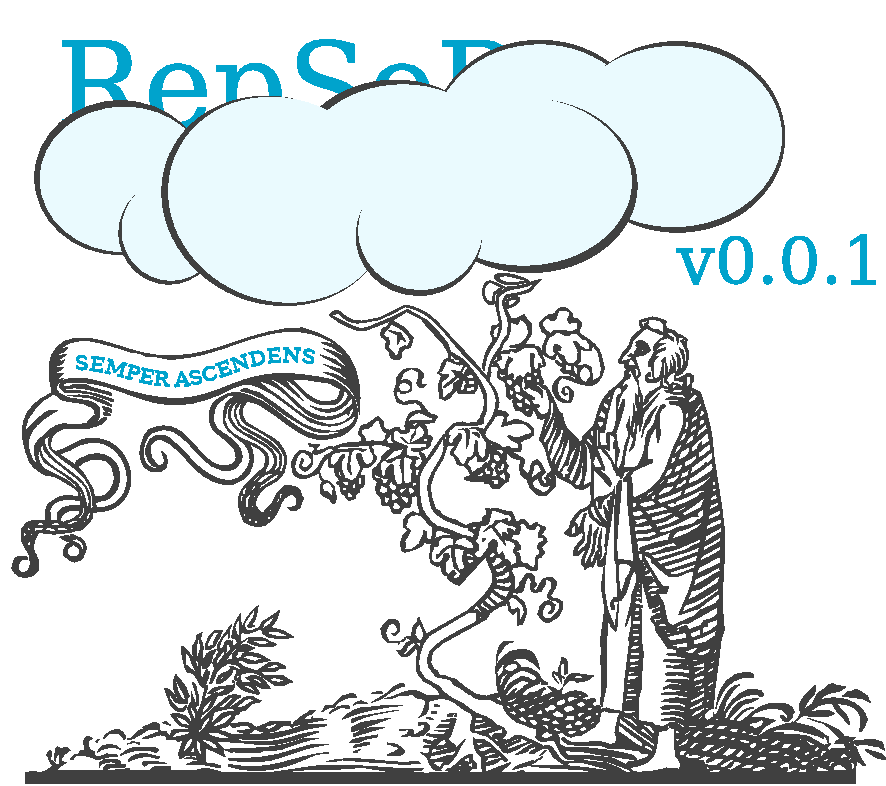
\includegraphics[width=0.8\textwidth]{img/repsep.pdf}
					\end{figure}
				\end{minipage}
			\end{frame}
\end{document}
